 \documentclass[letterpaper,11pt]{amsart}
\textwidth=16.00cm 
\textheight=22.00cm 
\topmargin=0.00cm
\oddsidemargin=0.00cm 
\evensidemargin=0.00cm 
\headheight=0cm 
\headsep=0.5cm

\textheight=610pt

\usepackage{latexsym,amsthm,amssymb,epsfig,url,tikz}%eufrak
%\usepackage[sumlimits]{amsmath}

\tikzstyle{vertex}=[circle, draw, inner sep=0pt, minimum size=6pt, fill]
\newcommand{\vertex}{\node[vertex]}

% \usepackage[centredisplay,PostScript=dvips]{diagrams}
%\usepackage[dvips]{color}
%\usepackage[mathscr]{eucal}mathrsfs

% Theorem Formatting Commands.
\theoremstyle{plain}
\newtheorem{thm}{Theorem}
%\newtheorem{lemma}{Lemma}[section]
\newtheorem{lemma}[thm]{Lemma}
\newtheorem{prop}[thm]{Proposition}
\newtheorem{cor}[thm]{Corollary}
\newtheorem{conj}[thm]{Conjecture}
\newtheorem*{thm*}{Theorem}
\newtheorem*{lemma*}{Lemma}
\newtheorem*{prop*}{Proposition}
\newtheorem*{cor*}{Corollary}
\newtheorem*{conj*}{Conjecture}

\theoremstyle{definition}
\newtheorem{defn}[thm]{Definition}
\newtheorem*{defn*}{Definition}
\newtheorem{ex}[thm]{Example}
\newtheorem{pr}{Problem}
\newtheorem{alg}[thm]{Algorithm}
\newtheorem{ques}[thm]{Question}

\theoremstyle{remark}
\newtheorem*{rmk}{Remark}
\newtheorem*{obs}{Observation}

\usepackage{color}
\newcommand{\dbfeedback}[1]{{\color{red} DB Feedback: #1}}

\newcommand{\conv}{{\rm Conv}}
\newcommand{\aff}{{\rm Aff}}
\newcommand{\rb}{{\rm rb}}
\newcommand{\ri}{{\rm relint}}
\newcommand{\rank}{{\rm rank}}



\begin{document}

\Large

\begin{center}
{\bf Math 7760 -- Homework  3 --  Due:  September 14, 2022}
\end{center}

\normalsize


\bigskip

\noindent {\bf Practice Problems:}

\bigskip

\begin{pr}
    Show that the standard cube and the standard cross polytope are polar duals of each other.
\end{pr}

\begin{pr}\label{pr: least upper bounds are unique}
    Show that least upper bounds and greatest lower bounds in a poset are unique.
\end{pr}

\begin{pr}\label{pr: lattices have zero-hats and one-hats}
    Prove that every finite lattice has a $\hat{0}$ and $\hat{1}$.
\end{pr}

\begin{pr}
    For each of the following posets, determine which are lattices.
    Among those that are, determine which are atomic and/or coatomic.\\
    \begin{center}
        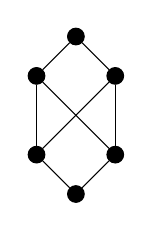
\begin{tikzpicture}
            \vertex (a) at (0,0){};
            \vertex (b) at (1,0){};
            \vertex (c) at (0,1){};
            \vertex (d) at (1,1){};
            \vertex (0) at (0.5,-0.5){};
            \vertex (1) at (0.5,1.5){};
            \path
                (a) edge (c) edge (d)
                (b) edge (c) edge (d)
                (0) edge (a) edge (b)
                (1) edge (c) edge (d)
            ;
        \end{tikzpicture}\qquad\qquad\qquad
        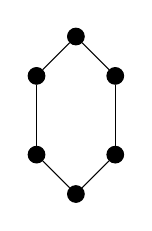
\begin{tikzpicture}
            \vertex (a) at (0,0){};
            \vertex (b) at (1,0){};
            \vertex (c) at (0,1){};
            \vertex (d) at (1,1){};
            \vertex (0) at (0.5,-0.5){};
            \vertex (1) at (0.5,1.5){};
            \path
                (a) edge (c)
                (b) edge (d)
                (0) edge (a) edge (b)
                (1) edge (c) edge (d)
            ;
        \end{tikzpicture}\qquad\qquad\qquad
        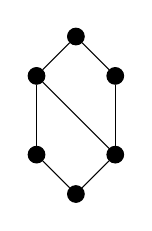
\begin{tikzpicture}
            \vertex (a) at (0,0){};
            \vertex (b) at (1,0){};
            \vertex (c) at (0,1){};
            \vertex (d) at (1,1){};
            \vertex (0) at (0.5,-0.5){};
            \vertex (1) at (0.5,1.5){};
            \path
                (a) edge (c)
                (b) edge (c) edge (d)
                (0) edge (a) edge (b)
                (1) edge (c) edge (d)
            ;
        \end{tikzpicture}\qquad\qquad\qquad
        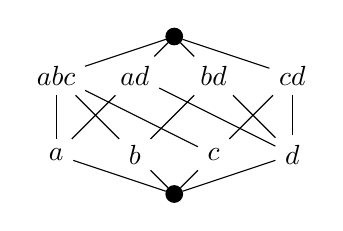
\begin{tikzpicture}
            \node (a) at (0,0){$a$};
            \node (b) at (1,0){$b$};
            \node (c) at (2,0){$c$};
            \node (d) at (3,0){$d$};
            \node (abc) at (0,1){$abc$};
            \node (ad) at (1,1){$ad$};
            \node (bd) at (2,1){$bd$};
            \node (cd) at (3,1){$cd$};
            \vertex (0) at (1.5,-0.5){};
            \vertex (1) at (1.5,1.5){};
            \path
                (0) edge (a) edge (b) edge (c) edge (d)
                (abc) edge (a) edge (b) edge (c)
                (ad) edge (a) edge (d)
                (bd) edge (b) edge (d)
                (cd) edge (c) edge (d)
                (1) edge (abc) edge (ad) edge (bd) edge (cd)
            ;
        \end{tikzpicture}
    \end{center}
\end{pr}

\begin{pr}\label{pr: algebraic definition of lattice}
    An \emph{algebraic lattice} consists of a set $S$ and two binary operations $\vee$ and $\wedge$ satisfying the following two axioms:
    \begin{enumerate}
        \item $x \vee (y \vee z) = (x \vee y) \vee z$ and $x \wedge (y \wedge z) = (x \wedge y) \wedge z$ for all $x,y,z \in S$ (associativity)
        \item $x \vee (x \wedge y) = x$ and $x \wedge (x \vee y)$ for all $x, y \in S$ (absorption).
    \end{enumerate}
    Show that if $(S,\le)$ is a lattice with join and meet operations $\vee$ and $\wedge$, then $(S,\vee,\wedge)$ is an algebraic lattice.
    Then, show that if $(S,\vee,\wedge)$ is an algebraic lattice,
    then there exists a partial order $\le$ on $S$ that is a lattice with meet and join operations $\vee$ and $\wedge$.
\end{pr}

\bigskip

\noindent {\bf Problems to write up:}

\bigskip

\begin{pr}
    Prove each of the following statements. 
    \begin{enumerate}
        \item The intersection of two polytopes is a polytope.
        \item The sum of two polytopes is a polytope.
        \item Every face of a polytope is exposed.
    \end{enumerate}
\end{pr}


\begin{pr}\label{pr: divisor lattice}
    Define a partial order $\prec$ on $\mathbb{N}$ by $x \prec y$ if and only if every prime divisor of $x$ is a prime divisor of $y$.
    \begin{enumerate}
        \item Show that $(\mathbb{N},\prec)$ is a lattice. What are the more familiar names for the meet and join operations?
        \item Does $(\mathbb{N},\prec)$ have a $\hat{0}$ and/or a $\hat{1}$? If applicable, determine its atoms/coatoms.
        \item Is $(\mathbb{N},\prec)$ atomic and/or coatomic?
        \item Show that $(\mathbb{N},\prec)$ is isomorphic to the poset $(S,\subseteq)$ where $S$ is the set of all finite multisets with elements in $\mathbb{N}$, partially ordered by inclusion.
    \end{enumerate}
\end{pr}

\begin{pr}
    Show that every polytope is affinely isomorphic to a bounded intersection of an orthant with an affine space.
\end{pr}

% \begin{pr}
%     Given $x,y \in \mathbb{R}^d$, we use the shorthand $x \ge y$ to mean that $x_i \ge y_i$ for all $i$.
%     Use the hyperplane separation theorem to prove (one of many versions of) the \emph{Farkas Lemma}:
%     \begin{lemma}
%         Let $A \in \mathbb{R}^{m\times d}$ and let $z \in \mathbb{R}^m$.
%         Then there exists a point $x \in \mathbb{R}^d$ with $Ax = 0$ and $x \ge 0$,
%         or there exists a row vector $c \in (\mathbb{R}^m)^*$ with $cA \ge 0$ and $cz < 0$,
%         but not both.
%     \end{lemma}
%     There are two other versions of the Farkas lemma in Ziegler's book (the one above also appears as version 2).
%     Convince yourself that they are indeed equivalent to the one above (no need to write anything up for it).
% \end{pr}







\end{document}